\chapter{Introduction}
\begin{refsection}

{\itshape
Here we will provide an overview of the following chapters as well as define the theoretical and experimental background for this work. 
The first section will be dedicated to the outline of this thesis, to aid the readers. 
A somewhat shallow review of the particle physics searches at PSI will follow, with some in-depth dive into the subjects which are close to the core of this thesis. 
This will be complemented by the description of the different facilities at PSI, with a final section dedicated to the Proton Ionization Facility. 
This whole chapter relies heavily on references \cite{Signorelli} \cite{PSI:review:2021}.}

\section{Outline of this thesis}
    The structure of this Thesis might differ slightly from the norm. While most of my colleagues dedicated their work to a singular subject, like a particular detector or theory, my effort during the course of my Ph.D. has been spread on a wider angle.
    At first glance, this work might seem the result of three separate projects, namely MEG MuEDM, and muCool. In fact, the spirit in which this Thesis has been written is orthogonal to the chapters themselves: the overall progress of muonic particle physics experiments.

    \begin{itemize}
        \item MEG
        \begin{itemize}
            \item how to use a CW
            \item Cryogenic and LH2
            \item data taking and analysis X17
        \end{itemize}
        \item MuEDM
        \begin{itemize}
            \item how to use Geant4
            \item beam insertion
            \item (beam time + analysis to check Geant4)
        \end{itemize}
        \item muCool
        \begin{itemize}
            \item field simulations for mu+ Transvers+Longitudinal
            \item begin of the study for mu-
        \end{itemize}
    \end{itemize}

\section{Particle physics at Paul Scherrer Institute}
    
\section{Bite-size theory}
    The aim of this section is to define the framework in which (part) of particle physics research is moving. In particular, we will be focusing on the aspects which are relevant to the three experiments core of this thesis.
    The searches \gls{bsm} proceed in two main directions: \textit{Intensity frontier} is used to describe the test of contributions which are too small to be experimentally accessible observing large numbers of events;
    \textit{Precision frontier} is used when improving the accuracy of a specific parameter to test the agreement with the \gls{sm}.
    Searches for \gls{clfv} or neutron \gls{edm} are examples of the former type while precision \gls{qed} tests with muonium are of the latter.
    
    \subsection{Standard Model at low energies}
        In the low energy regime \gls{qed} and \gls{qcd} are essentially `frozen', and the \gls{sm} reduces to the standard Lagrangian
        \begin{equation}
            \mathcal{L}_{QED+QCD}=\sum_{f}\bar{f}(i\cancel{D}-m_f)f-\frac{1}{4}F_{\alpha\beta}F^{\alpha\beta}-\frac{1}{4}G_{\alpha\beta}G^{\alpha\beta}
            \label{eq:sm}
        \end{equation}
        where $F$ and $G$ are the electromagnetic and gluonic field-strenght tensors. The sum here is on fermions of mass $m_f$, charge $eQ_f$ and color $g_st^a_f$. For a lepton this would mean $Q_\ell=-1$ and $t^a_\ell=0$ while for a quark $Q_q=2/3$ or $-1/3$ and $t^a_q=\lambda^a/2$, with $\lambda$ Gell-Mann matrices.
        To compute the matrix element between two lepton states we find:
        \begin{equation}
            \matrixel{\ell(p_2)}{J^a_{em}}{\ell(p_1)} =\bar{u}(p_2,m_\ell)\left(F^{(\ell)}_1(q^2)\gamma^a+F^{(\ell)}_2(q^2)\frac{i\sigma^{\alpha\beta}q_\beta}{2m_\ell} \right)u(p_1,m_\ell)
            \label{eq:matrix}
        \end{equation}
        Here $u$ and $\bar{u}$ are the spinors and the two states are with momenta $p_1$ and $p_2=p_1+q$ while $F_1^{(\ell)}$ and $F_1^{(\ell)}$ are related rispectively to the electric charge and the \gls{amm}. 
        In particular, fort the \gls{amm} we find
        \begin{equation}
            F_2^{(\ell)}(0) = a_\ell = \frac{(g-2)_\ell}{2}  
            \label{eq:amm}
        \end{equation}
        Even when considering non point-like particles, like nucleons $N\in \{p,n\}$ the form used in \ref{eq:matrix} holds and we find:
        \begin{equation}
            \matrixel{N(p_2)}{J^a_{em}}{N(p_1)} =\bar{u}(p_2,m_N)\left(F^{(N)}_1(Q^2)\gamma^a+F^{(N)}_2(Q^2)\frac{i\sigma^{\alpha\beta}q_\beta}{2m_N} \right)u(p_1,m_N)
        \end{equation}
        Here $Q^2\equiv -q^2$ and, while \ref{eq:amm} holds, $F_2^{(N)}$ depends on strong dynamics.
        In the case of nucleons, it is often useful to introduce the \textit{electric} and \textit{magnetic form factors}
        \begin{equation*}
            G^{(N)}_E(Q^2)\equiv F_1^{(N)}(Q^2)-\frac{Q^2}{4m_N^2}F_2^{(N)}(Q^2);
            \quad 
            G^{(N)}_M(Q^2)\equiv F_1^{(N)}(Q^2)+F_2^{(N)}(Q^2)
        \end{equation*}
        It is of particular interest that, in the limit for small $Q^2$, the form factors can be understood as Fourier transform of extended classical `charge' distributions $\rho_i(r)$
        \begin{equation*}
            F_i(Q^2) = \int \dd[3]\bm{r}e^{-i\bm{q\cdot r}}\rho_i(r) = \int \dd[3]\bm{r}\rho_i(r) +\frac{1}{6}Q^2 \int \dd[3]\bm{r}r^2\rho_i(r)  + \dots
        \end{equation*}
        From this, we can write the general expression for the second moment of the charge distribution or \gls{edm}. This relation is used for example when determining the charge and magnetic radii of the proton.
        \begin{equation}
            r^2_i\equiv\frac{1}{N}\int \dd[3]\bm{r}r^2\rho_i(r) = -6\frac{1}{N}\evaluated{\frac{dF_i(Q^2)}{dQ^2}}_{Q^2=0};
            \quad
            N=\begin{cases}
            1 & \text{if}\ F_i(0)=0,\\
            F_i(0) &\text{else}.
            \end{cases}
        \end{equation}
        When introducing the weak interaction we arrange fermions in \textit{left-handed doublets} and \textit{right-handed singlets}.
        We then define the \textit{charged weak current} $J_{cc}^\alpha$, a similar \textit{neutral weak current} $J_{cn}^\alpha$ and we find
        \begin{equation}
            \mathcal{L}_{EW}=eA_\alpha J_{em}^\alpha + \frac{g}{\sqrt{2}}\left(W^+_\alpha J_{cc}^\alpha+\text{h.c.} \right) + g_zZ_\alpha J^\alpha_{nc};
            \quad
            J^\alpha_{cc}=\sum_\ell \bar{\nu}_\ell\gamma^\alpha P_L\ell+\sum_{ij}V_{ij}\bar{u}_i\gamma^\alpha P_L d_j
        \end{equation}
        where $g=e/\sin{\vartheta_W}$, $g_Z=e/\cos{\vartheta_W}$ are the $SU(2)_L$ coupling  expressed trough the Weinberg mixing angle $\vartheta_W$. Only the left handed fermions are coupled (trought $P_L\equiv (1-\gamma_5)/2$) and in the sum over the quark the \gls{ckm} matrix $V_{ij}$ describes the flavor-changing effect.
        When dealing with masses much smaller than $m_W$ and $m_Z$ the result is the `effective' Fermi theory current-current interaction
        \begin{equation}
            \mathcal{L}_{4F}= -\frac{4 G_F}{\sqrt{2}} \left( J_{cc}^\alpha(J_{cc})^\dag_\alpha + J^\alpha_{nc}(J^\alpha_{nc})_\alpha\right)
        \end{equation}
        In this equation $4G_F/\sqrt{2}=g^2/(2m_W^2)$ and using the definitions for $J_{nc/cc}^\alpha$ we end up with the vector contact interactions.
        In this framework photons and gluons are the only gauge bosons and the gauge symmetry of the \gls{sm} $SU(3)_c\times SU(2)_L\times U(1)_Y$ is reduced to \gls{qcd} and \gls{qed}: $SU(3)_c\times U(1)_{em}$.
        We can write a 6-dimension vector operator which links 4 fermions in a generic form
        \begin{equation}
            [O^{XY}_{f}]_{ijkl}=(\bar{\psi}_i\gamma^\alpha P_X \psi_j)(\bar{\psi}_k\gamma_\alpha P_Y \psi_l)
        \end{equation}
        where $X,Y \in {L,R}$ and ${i,j,k,l}$ are generation indices. There are many such operators because $\psi$ could be leptons or quarks but the integration of the $W$ and $Z$ generates only a subset (i.g. we have no \gls{clfv} operator due to accidental symmetries).
        In a similar fashion an operator will be a 6-dimension scalar when removing the $\gamma$ matrices or a 5-dimension dipole operators including photons and gluons:
        \begin{equation}
            [O^D_{f\gamma}]_{ij}=(\bar{\psi}_i\sigma_{\alpha\beta}P_R\psi_j)F^{\alpha\beta};
            \quad
            [O^D_{qG}]_{ij}=(\bar{\psi}_i\sigma_{\alpha\beta}G^{\alpha\beta}P_R\psi_j)
        \end{equation}
    
    \subsection{Beyond Standard Model at low-energy}
        There is no shortage of \gls{bsm} models and one way of (roughly) classifying them would be by the masses and coupling strengths of the particles they introduce. 
        Light \gls{bsm} particles have small couplings to \gls{sm} particles, which would explain the small contribution to physical observables. Prominent examples are dark photons, axions and \gls{alp}.
        Axions in particular were proposed as a solution to the small value of the \gls{cp} violating \gls{qcd} $\vartheta$ parameter.
        When discussing Heavy \gls{bsm} particles we can follow the process of `integration' shown for $W$ and $Z$ in this section, in an \gls{eft} approach.
        As long as the \gls{bsm} physics respects \gls{qed} and \gls{qcd} gauge symmetry and involves `large' mass scale $\Lambda$ ($m_b<\lambda<m_W$), it can be integrated out. 
        This way we add higher-dimensional operators to the \gls{sm} Lagrangian, obtaining a \gls{left}
        \begin{equation}
            \mathcal{L}_{LEFT}=\mathcal{L}_{QED+QCD}+\frac{1}{\Lambda}\sum_iC^{(5)}_iO^{(5)}_i +\frac{1}{\Lambda^2}\sum_iC^{(6)}_iO^{(6)}_i +\dots
            \label{eq:left}
        \end{equation}
        Parameterize low-energy observables and measuring (or constraining) associated parameters is not easy task: a prime example would be the Michel decay (which we will discuss in the following sections), generalized in terms of scalar vector and tensor contact interactions or the similar effort for the \gls{clfv} $\mu\rightarrow e \gamma$ and $\mu \rightarrow eee$ withe lepton-flavour-violating contact interactions.
        
        If the \gls{bsm} physics appears at a scale larger than $m_W$, we first have to develop a \gls{smeft}.
        The details on how this is achieved are outside our purpose but including all the different gauge fields, higgs doublet, left-handed doublets and right-handed singlet (respecting the $SU(3)_c\times SU(2)_L\times U(1)_Y$ gauge symmetry) we find
        \begin{equation}
            \mathcal{L}_{SMEFT}=\mathcal{L}_{SM}+\frac{1}{\Lambda}(C^{(5)}O^{(5)}+\text{h.c.}) +\frac{1}{\Lambda^2}\sum_iC^{(6)}_iO^{(6)}_i +\dots
            \label{eq:smeft}
        \end{equation}
        
        We can now re-evaluate the matrix in \ref{eq:matrix} element using \ref{eq:smeft} instead of \ref{eq:sm}.
        We will leave the details of the calculation under the hood but the result we get is the following
        \begin{equation}
        \begin{split}
            \matrixel{f(p_2)}{J^\alpha_{em}}{f(p_1)} = 
            \bar{u}(p_2,m_f) \left(F^{(f)}_1(q^2)\gamma^a+ \left(F^{(f)}_2(q^2)- i\gamma_5F^{(f)}_3(q^2)\right) \frac{i\sigma^{\alpha\beta}q_\beta}{2m_f}+ \right.\\
            \left. F^{(f)}_4(q^2)\frac{1}{m_f^2}(q^2\gamma^\alpha-2m_fq^\alpha)\gamma_5 \right) u(p_1,m_f)
        \end{split}
        \end{equation}
        It is of interest that the \gls{cp}-violating $F_3$ form factor is linked to the \gls{edm} of the lepton $d_f$
        \begin{equation}
            d_f=\frac{eF_3^{(f)}(0)}{2m_f}
            \label{eq:edm}
        \end{equation}
        In the \gls{sm}, $d_f$ recives contributions from quarks at 3-loops and leptons at 4-loops (induced by \gls{cp}-violation in the \gls{ckm}). When considering protons and neutrons there is an additional contribution from the \gls{cp} violating \gls{qcd} $\vartheta$ parameter (found to be extremely low constraining the neutron \gls{edm}).
        For completeness sake, $J_{cc}^\alpha$ give rise to matrix elements between different $SU(2)$ doublets, like $(\nu_\ell,\ell)$ or $(p,n)$. This leads to muon and beta decay or quasi-elastic scattering $\ell p\rightarrow \nu_\ell n$.

    \subsection{Muon}
        The muon is the lepton with the intermediate mass of $m_\mu \approx 105.66$ MeV and it is unstable. The dominant process is the Michel decaly $\mu\rightarrow e\nu\bar{\nu}$ which translates to a lifetime of $\tau\approx2.2\ \mu$s. We already hinted to the fact that the this decay is mediated by the charged current $J_{cc}^\alpha$ through $\matrixel{\nu_\mu}{J_{cc}^\alpha}{\mu}\matrixel{e}{(J_{cc})^\dag_\alpha}{\nu_e}$ which in \gls{eft} corresponds to $(\bar{\nu}_\mu\gamma^\alpha P_L\mu)(\bar{e}\gamma_\alpha P_L\nu_e)$. The resulting \gls{eft} Lagrangian is
        \begin{equation}
            \mathcal{L}_{Fermi}=-\frac{4G_F}{\sqrt{2}} (\bar{\nu}_\mu\gamma^\alpha P_L\mu)(\bar{e}\gamma_\alpha P_L\nu_e) + \text{h.h}+ \mathcal{L}_{QED+QCD}
        \end{equation}
        When evaluating the lifetime we get an equation which contains, in $\Delta q$, all corrections induced by our Lagrangian: electron mass effect, higher odred \gls{qed} correction and hadronic corrections. 
        \begin{equation}
            \frac{1}{\tau_\mu}\equiv\Gamma_\mu = \Gamma_0(1+\Delta q) = \frac{G_F^2 m_\mu^5}{192 \pi^3}(1+\Delta q)
            \label{eq:tau}
        \end{equation}
        Unfortunately, \gls{qcd} corrections are non-perturbative for $q^2\sim m_\mu^2$ and are the leading theoretical uncertainty. These correction are known at NNLO.
        Precision measurement of the muon lifetime is key for consistency checks of th \gls{sm}. In fact $G_F$ can be relate to $m_W$ and $m_Z$
        \begin{equation}
            \frac{4G_F}{\sqrt{2}}=\frac{g^2}{2m_W^2}(1+\Delta r)=\frac{2\pi}{\sin^2\vartheta_Wm_W^2}(\+\Delta r)
        \end{equation}
        Here $\Delta r$ are the \gls{sm} corrections and $\sin^2\vartheta_W=1-m_W^2/m_Z^2$.\\
        On top of the Michel decay we also have radiative and rare decays
        \begin{equation}
            \mu\rightarrow e\nu\bar{\nu}\gamma, \quad \mu\rightarrow e\nu\bar{\nu}e^+e^-
        \end{equation}
        for which we have $B(\mu\rightarrow e\nu\bar{\nu}\gamma)\sim 1.3\times 10^{-2}$ (for $E_\gamma>10$ MeV) and $B(\mu\rightarrow e\nu\bar{\nu}ee)\sim 3.6 \times 10^{-5}$.
        
                 At last we arrive to the `golden' channels for \gls{clfv} studies:
        \begin{equation}
            \mu\rightarrow e\gamma, \quad \mu\rightarrow eee, \quad \mu^- \ ^A_ZN\rightarrow e^-\ ^A_ZN
        \end{equation}
        With non-vanishing neutrino masses, the branching rations for these processes are expected to be below $10^{-50}$.
        To extract constraints on \gls{bsm} physics from the branching rations we can mostly use standard pertuvbative methods with the Lagrangian \ref{eq:left}.
        For the muon conversion additional precautions are needed due to the nuclear matrix elements $\matrixel{^A_ZN}{J}{^A_ZN}$ as well as the study of the \gls{dio}, electrons for which the energy spectrum was is modify by the nuclear recoil.
        
        The last two properities of interest of the muon are the \gls{amm} (eq. \ref{eq:amm}) and \gls{edm} (eq. \ref{eq:edm}). 
        After the results of the G-2 experiment at \gls{fnal} there is some tension on the first between experimnetal results and theory. 
        For the \gls{edm} the \gls{sm} value is zero for practical purposes and a non-vanishing result would be clear indication of \gls{bsm}.
        We will further discuss the muon \gls{edm}.
        
    \subsection{Muon decay}
        When using a charge-changing Hamiltonian characterized by fields with define chirality \cite{5}, the general matrix element of the muon decay can be written as \cite{7}
        \begin{equation}
            M=4\frac{G_F}{\sqrt{2}}\sum_{\substack{ \gamma = S,V,T \\ \varepsilon,\mu = R,L}}g^\gamma_{\varepsilon\mu} \matrixel{\bar{e}_\varepsilon}{\Gamma^\gamma}{(\nu_e)_n} \matrixel{(\bar{\nu}_\mu)_m}{\Gamma_\gamma}{\mu_\mu}
        \end{equation}
        In this definition we find: $\gamma$ indicates a 4-scalar, 4-vector or 4-tensor; $\Gamma$ Dirac (or Pauli) matrices; $\varepsilon$, $\mu$ indicate the chirality of the spinors; m, n the chirality of the neutrinos.
        This means that the physical interpretation of $g^\gamma_{\varepsilon\mu}$ is quite straightforward: $n_\gamma|g^\gamma_{\varepsilon\mu}|^2$ is the probabilit of a $\mu$-handed muon decaying in a $\varepsilon$-handed electron by the interaction $\Gamma^\gamma$ ($n_\gamma$ are required for the correct normalization).
        In this picture the \gls{sm} corresponds to $g_{LL}^V=1$ with all other couplings to 0. 
        \textcolor{red}{Review chirality vs helicity}
        
        \paragraph{Observables}
        Neglecting radiative corrections, we find the differential decay probability with: reduced energy in $[x,x+\dd x]$; along $\hat{x}_3$ with an angle $[\vartheta,\vartheta+\dd\vartheta]$ with respect to the muon polarization $\pmb{P}_\mu$; spin along $\bm{\hat{\zeta}}$.
        
        \begin{equation}
           \pdv[2]{\Gamma}{x}{\cos\vartheta}=\frac{m_\mu}{4\pi^3}W^4_{e\mu}G^2_F\sqrt{x^2-x_0^2}\cdot \{F_{IS}(x)\pm P_\mu\cos\vartheta F_{AS}(x)\}\cdot\{\bm{\hat{\zeta}\cdot P}_e(x,\vartheta)\}
           \label{eq:differentialdecay}
        \end{equation}
        
        Here, $W_{e\mu}=max(E_e)=(m_\mu^2+m_e^2)/2m_\mu$ is the maximum $e^\pm$ energy and $x=E_e/W_{e\mu}$ is the reduced energy ($x_0=m_e/W_{e\mu}$).
        This spectrum has both an isotropic ($F_{IS}$) and anisotropic part ($F_{AS}$). 
        The electron polarization $\bm{P}_e(x,\vartheta)$ can be parametrized by \textit{Michel parameters}, which are combinations of the coupling constants $g^\gamma_{e\mu}$.
        If the neutrinos'  and $x_0$ are neglected, \ref{eq:differentialdecay} becomes
        \begin{equation}
            \pdv[2]{\Gamma}{x}{\cos\vartheta}\sim x^2\left\{ 3(1-x)+\frac{2\rho}{3}(4x-3)+3\eta x_0\frac{(1-x)}{x} \pm P_\mu\xi\cos\vartheta  \left[1-x+\frac{2\delta}{3}(4x-3) \right]\right\}
        \end{equation}
        Here $\vartheta$ is the angle between the elctron momentum and the muon spin and $x\equiv2E_e/m_\mu$. 
        In the \gls{sm} we get the following, in which we find the total rate used in \ref{eq:tau}. \textcolor{red}{$\rho=\xi\delta=3/4$, $\xi=1$, $\eta=0$}
        \begin{equation}
            \pdv[2]{\Gamma}{x}{\cos\vartheta}=\frac{G_F^2 m_\mu^5}{192 \pi^3} \left[ 3-2x \pm P_\mu\cos\vartheta (2x-1) \right]x^2
        \end{equation}

        The way the $g^\gamma_{e\mu}$ are connected to the nine decay parameters \cite{3,10}, or the 10 intermediate quantities we can measured \cite{3}, is outside the purpose of this short review. 
        The bottom line is that a 20-dimensional space of the complex $g^\gamma_{e\mu}$ can be mapped to a 10-dimensional space.
        Unfortunately many of these parameters are intertwine and (generally) the precise measurement of individual parameters does not give conclusive information on the type of interaction.
        
        To avoid being too vague we will take an example from \cite{PSI:review:2021}. 
        The rate $S$ of the reaction $\nu_\mu e^-\rightarrow \mu^-\nu_e$, normalized to the rate predicted by $V-A$ and assuming a negative helicity for $\nu_\mu$, has been found close to 1 \cite{17}.
        $S$ depends on five coupling constants $\{g^v_{LL},g^v_{RL},g^s_{LR},g^s_{RR}\}$ but four of these parameters are found to be small, and in first approximation we find \cite{7}:
        \begin{equation}
            S=|g^v_{LL}|^2; \quad |g^s_{LL}|<2\sqrt{1-S}
        \end{equation}
    \subsection{Experiments}
    \paragraph{Longitudinal Positron Polarization}
    \paragraph{Transverse Positron Polarization}
    \paragraph{Electron Decay Asymmetry}
    
    \subsection{Electric Dipole Moment}
        \label{intro:edm}
        Similarly to how the \gls{mdm} $\mu$ represents the coupling between the spin of a quantum system and an external magnetic $\bm{B}$ field, the \gls{edm} $d$ represents the coupling between the spin of and an external electric field $\bm{E}$.
        The Hamiltonian describing the spin dynamics, indicating the Pauli matrices with $\bm{\sigma}$, is then:
        \begin{equation}
            \hat{H} = -\mu\bm{\hat{\sigma}\cdot B}-d\bm{\hat{\sigma}\cdot E}
        \end{equation}
        Given that $\bm{\hat{\sigma}\cdot E}$ is odd for time reversal, the existence of a non-zero \gls{edm} would violate \gls{cp} symmetry. 
        This is an interesting topic, with many implications and key to meany searches. 
        Here we will just nominate it and underline that at \gls{psi} has been for decades at the frontier in the measurements of the neutron \gls{edm}.
        We will discuss the muon \gls{edm} in detail in the chapter dedicated to the \gls{muedm} experiment.\\
\cite{edmasprobe}
\section{Experimental status}
    \subsection{MEG}
    \subsection{Mu3e}
    \subsection{Mu2e}
    \subsection{COMET}
    \subsection{nEDM}
    \cite{n2EDM}    
    \subsection{MUSE}
    \subsection{MuX}

\section{The beams at PSI}
    \label{intro:beamlines}
    \subsection{High Intensity Proton Accelerator Facility}
    \label{sec:hipa}
    The source of the particle beams at PSI is the \gls{hipa}, which produces a proton beam up to 1.4 MW at 590 MeV of kinetic energy.
    A Isochronous proton cyclotron  is the main accelerator, with 8 magnet sectors and 4 accelerating cavities at 50.6 MHz.
    
    \begin{figure}
        \centering
        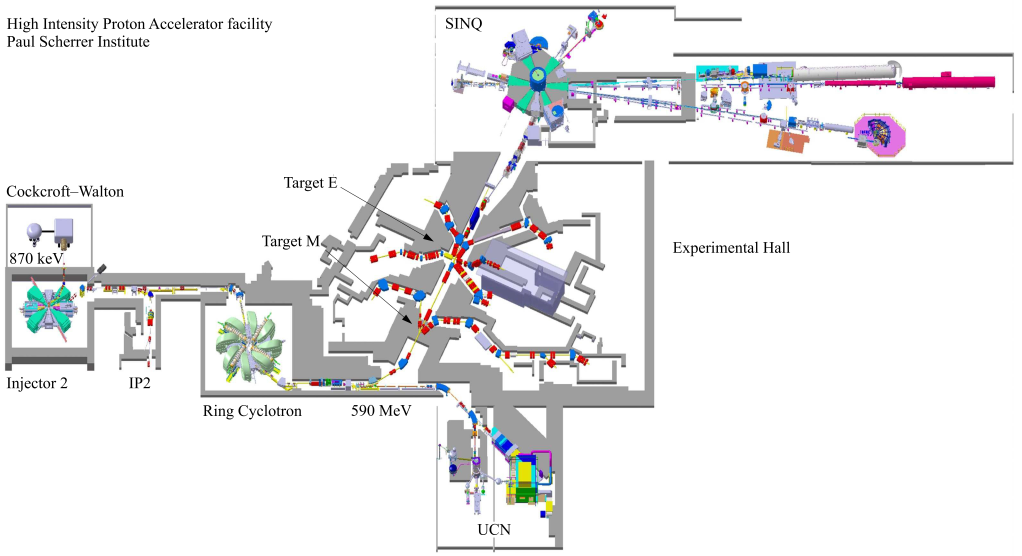
\includegraphics[width = \textwidth]{Figures/Introduction/PSI_HIPA.png}
        \caption{\acrfull{hipa} facility at PSI}
        \label{fig:PSI:HIPA}
    \end{figure}
    \paragraph{Pions and Muons production}
    \paragraph{Neutron production}
    \paragraph{Isotope production}
        
    \subsection{Meson production}
        As we saw in \ref{sec:hipa}, \gls{hipa} delivers a continuous $2.4$ mA $590$ MeV proton beam. 
        To have a high pion/muon yield a low Z material is the best choice for the Meson Production Targets: graphite is has been used since 1990's.
        The whole system (target, collimators, beam dumps, \dots) has to be cooled and, due to nuclear reactions, is highly radioactive.
        Pions are produced by the interaction with nucleons in the target (threshold at 280 MeV in the center-of-mass frame) and muons are then produced by pion decay.
        When $\pi$ are stopped at $\sim 1$ mm from the surface of the target, $\mu^+$ can escape and are called \textit{surface muons}.
        These muons have energies below 4.1 MeV ($p=29.8$ MeV) and are $\approx100\%$ polarized.
        Muons created by in-flight decay have higher energies and are cooled \textit{cloud muons}. Both positive and negative muons are possible but the negative charge is suppressed by a factor $\sim 3$.
        There are two targets: M feeds two beamlimes (PiM1 and PiM3; E feeds 5 beamlines (PiE1, MuE1, MuE4, PiE3, PiE5).
        The targets are graphite wheels which rotate to distribute the heat due to the impinging beam.
        The material is polycrystalline graphite made of small crystallites of \SI{\sim20}{\mu m} irregularly arranged.
        
        \paragraph{E Target}
        The target is inserted vertically into the beamline and held by a horizontal rotating shaft. The graphite and the hub are connected by six spokes. 
        While operated at \SI{2}{mA}, the temperature of this \SI{40}{mm}/\SI{60}{mm} target is \SI{\sim1700}{K}. Water-cooled copper shields are mounted on the rear of the target. To reduce the deformations the graphite rim is made of 12 segments. 
        Variations of the beam positions are crucial and to improve the sensitivity the graphite wheel was modified: small grooves were applied on both sides. This modulates the beam transmission.
        At the end of 2019 a new target wheel was tested, having a small angle for the impinging beam. 
        This \textit{slanted target} keeps the effective thickness creating a larger active surface and two different spots for IN/OUT of the beam. The net effect is an increase $\sim50\%$ in the surface muons.
        As the bearings degrade from heat and radiation they have to be replaced after a few months of operation. The procedure for the maintenance of the target here will not be discussed.
        
        \paragraph{M Target}
        This target is smaller in thickness and the bearings are far from the beam thus the demands are less challenging. 
        The rim of the target is \SI{2}{cm} wide and \SI{2}{mm} thick.  
        With an impinging angle of \SI{30}{\deg} the effective thickness is \SI{5.2}{mm} inducing a beam loss of $1.6\%$. 
        The target operates at \SI{1100}{K} and is cooled by conduction.
        For the upcoming \gls{himb} the aim is to increase the muon rate by a factor up to 100. 
        For this purpose studies for an upgrade of the M target station, with a slanted target design, are ongoing.
        A similar slanted target was already tested in the E target station, yielding a $\sim 50\%$ increase in surface muon rate.
        
        \paragraph{Collimators and Beam dump}
        Just like target E, Collimators and beam dump are inserted vertically and shielded.
        Both are made of oxygen-free copper: improve thermal conductivity; avoid hydrogen embrittlement        \footnote{Hydrogen can be produced by the spallation reaction of the protons with copper. This hydrogen can bond with oxygen creating water molecules which can produce cracks in the copper.}; for brazing of the steel tubes onto the copper body.
        To avoid any significant change in the material, the copper is kept below \SI{400}{K} using water-cooling.
        The collimator system as well as the beam dump have to stand more than 100 kW per component.
        The water flows in stainless steel pipes are wound outside and brazed on the cylindrical body. 
        This is done to avoid direct contact of the proton beam with the water, which would create corrosion-inducing ions.
        The main body is made of six slices brazed together.
        The shape and manufacture of these sections were optimized using computational fluid dynamics in order to reduce the energy deposit and thermal stress.
        An aperture, made of 4 slits of \SI{100}{\mu m} Nikel foils, is mounted in front of the devices.
        Here free electrons from ionization are collected and used for beam position and size monitoring.
        Aside from a water leak problem, likely due to thermal stress, no visible signs of radiation damage are observed since installation.
\subsection{UltraCold Neutron source}
        Neutrons below \SI{4}{mK} are called UltraCold. 
        This corresponds to energy below \SI{300}{neV}, which is comparable with the gravitational potential of a neutron at a few meters height and the potential and also the neutron optical potential: material bottles can hence contain UCNs.
        The first spallation neutron source built at PSI was SINQ, which has dedicated neutron scattering instruments and was used as a polarized cold-neutron beam line for fundamental neutron physics.
        This beamline was used for many measurements conducted in preparation of the UCN source and many parameters of UCN production (and loss) were here determined.
        The design of the UCN source was presented in 2000 to push the sensitivity of the nEDM search.
        
        \paragraph{Source setup}
        The HIPA \SI{590}{MeV} proton beam is deflected by a magnetic kicker and sent in the spallation source.
        Each spallation reaction with the lead atoms leads to an average of 8 neutrons, which are then thermalized in heavy water.
        The main moderator is made of solid deuterium at \SI{5}{K}.
        The UCN produced exit the moderator's vessel through a thin aluminium lid in a vertical guide and their energy is lost to gravity.
        From here the UCN are delivered via  long neutron guides: two at the bottom and one at the top of the vessel.
        The 30 litres of solid D$_2$ is the core of the whole system and takes several days to achieve a good ice quality.
        UCN intensity reflects the quality of the achieved solid deuterium, as shown in shows the typical UCN intensity behaviour during such a slow freezing process.
        
        \paragraph{Performance}
        A key parameter in the performance of a UCN source is the number of particles delivered.
        The exponential decay measured at the lower ports reflects the emptying time of the central storage vessel.
        Measuring in the higher port a faster exponential is found, demonstrating that the UCNs with energies high enough to reach that port are quickly drained.
        Several studies to understand all aspects of the UCN source have been conducted since its inauguration, as well as the UCN transport from production in the solid deuterium to a beam port.
        A slow decrease in performance was discovered and studied and a temperature-cycling ``conditioning'' was developed to regain maximum UCN intensity.
        PSI UCN source has been reliably operating since 2011.

        \paragraph{Results}
        The resulting new nEDM limit was published in 2020 but other results were also obtained:
        \begin{itemize}
            \item A measurement of the mercury-to-neutron magnetic moment ratio
            \item Spin-echo spectroscopy with ultracold neutrons
            \item Measurement of gravitational depolarization of ultracold neutrons
            \item limit for oscillating electric dipole moments
            \item limit for spin-dependent forces mediated by axion-like particles
        \end{itemize}

        \begin{figure}
            \centering
            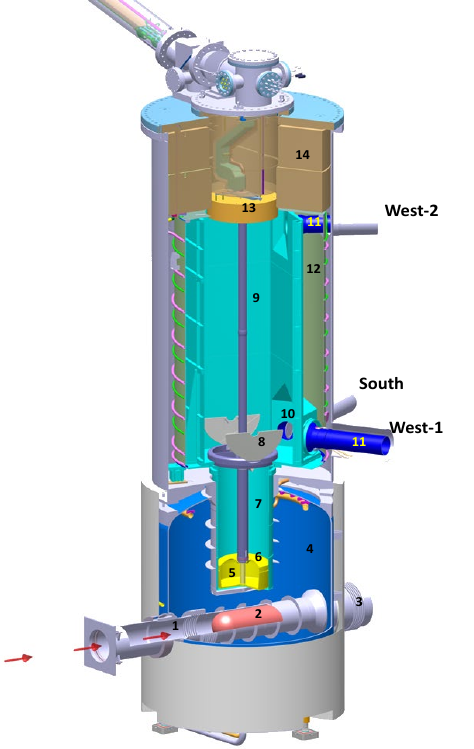
\includegraphics[scale = 0.5]{Figures/Introduction/UCN_CAD.png}
            \caption{CAD for the UCN source taken from  \cite{PSI:review:2021}. Some of the key aspects are: 2 - lead spallation source, 4 - heavy water moderator, 5 - D$_2$ moderator, 9 - storage vessel, 10 - 11 UCN guide and guide shutter.}
            \label{fig:UCN_CAD}
        \end{figure}
        \begin{figure}
            \centering
            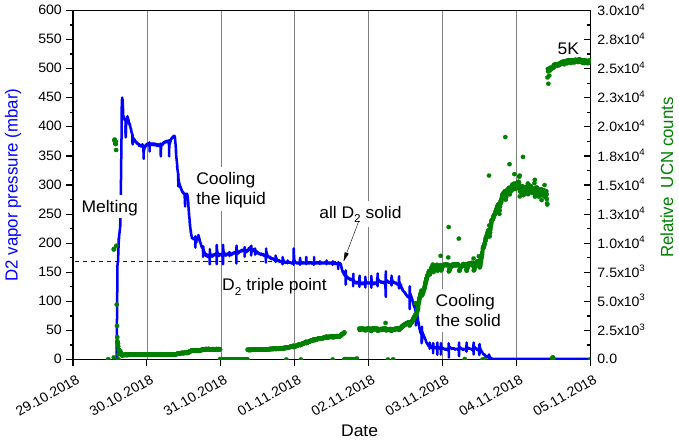
\includegraphics[scale = 0.5]{Figures/Introduction/UCN_behaviour.png}
            \caption{The observed behavior during the slow freezing of the deuterium. The large increase in UCN output shown by the green bullets
            demonstrates the strong reduction in UCN losses within the D$_2$. 
            Figure taken from \cite{PSI:review:2021}}
            \label{fig:UCN_behaviour}
        \end{figure}
        \begin{figure}
            \centering
            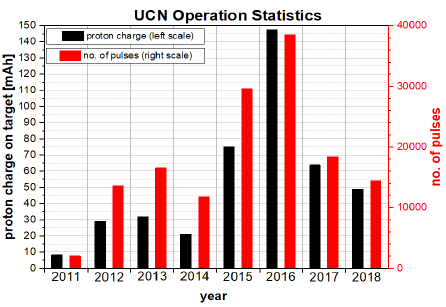
\includegraphics[scale = 0.5]{Figures/Introduction/UCN_stats.png}
            \caption{Annual statistics of the first operating years of the UCN source showing total accumulated beam current on target (black bars) and number of beam pulses (red bars) on the UCN spallation target. 
            Figure taken from \cite{PSI:review:2021}}
            \label{fig:UCN_stats}
        \end{figure}


    \subsection{Muon beam-line}
    \subsection{High-Intensity Muon Beams}
    \cite{HIMB:2021} 

\section{Proton Ionization Facility}
Another interesting facility at PSI is the Proton Ionization Facility (PIF)\cite{PIF:1996}\cite{PIF:2001}.
This was designed, in conjunction with the European Space Agency, to be a user-friendly testing ground for spacecraft components.
The deteriorating effect that high-energy protons can have on semiconductors is a key aspect of the correct functioning of spacecraft in the space environment.
Depending on the orbit and the duration of the flight the exposure to this hazard can vary and having reproducible test grounds is cardinal during the design phase. 
The original goals of this facility were:
\begin{outline}
\1 Radiation hardness of the new electronic products
\1 Single Event Upsets (SEU) and Latch-ups (SEL) of electronic components
\1 Properties of radiation monitors for space and laboratory applications
\1 Basic mechanics of radiation effects in semiconductors
\1 Space radiation environment by on-earth simulations
\end{outline}
Given the broad range of energy and intensities of the facility, alongside ESA many other users apply for beamtime at PIF within the accelerator communities such as CERN but also external laboratories, industries, and universities.
During the daytime, the beam is usually reserved for biomedical applications and these irradiation studies are done parasitically during the night and on weekends.
Although only for a short period, I joined PIF and I had the opportunity to be a shifter. 
It was quite an interesting experience, allowing me to become acquainted with a different setup and to see a different aspect of the research in particle physics.

\subsection{Facility and main features}

\addcontentsline{toc}{chapter}{Bibliography for the introduction}
\printbibliography[title=Bibliography for the introduction]
\end{refsection}